\documentclass[12pt,conference]{IEEEtran}




% *** GRAPHICS RELATED PACKAGES ***
%
\ifCLASSINFOpdf
  \usepackage[pdftex]{graphicx}
  % declare the path(s) where your graphic files are
  % \graphicspath{{../pdf/}{../jpeg/}}
  % and their extensions so you won't have to specify these with
  % every instance of \includegraphics
  % \DeclareGraphicsExtensions{.pdf,.jpeg,.png}
\else
  % or other class option (dvipsone, dvipdf, if not using dvips). graphicx
  % will default to the driver specified in the system graphics.cfg if no
  % driver is specified.
  % \usepackage[dvips]{graphicx}
  % declare the path(s) where your graphic files are
  % \graphicspath{{../eps/}}
  % and their extensions so you won't have to specify these with
  % every instance of \includegraphics
  % \DeclareGraphicsExtensions{.eps}
\fi
\hyphenation{op-tical net-works semi-conduc-tor}


\begin{document}
%
% paper title
% Titles are generally capitalized except for words such as a, an, and, as,
% at, but, by, for, in, nor, of, on, or, the, to and up, which are usually
% not capitalized unless they are the first or last word of the title.
% Linebreaks \\ can be used within to get better formatting as desired.
% Do not put math or special symbols in the title.
\title{Approximating Data Movement via Compiler Support}


% author names and affiliations
% use a multiple column layout for up to three different
% affiliations
\author{\IEEEauthorblockN{Junhan Zhou}
\IEEEauthorblockA{Carnegie Mellon University\\
Email: junhanz@andrew.cmu.edu}
\and
\IEEEauthorblockN{Vignesh Balaji}
\IEEEauthorblockA{Carnegie Mellon University\\
Email: vigneshb@andrew.cmu.edu}}



% make the title area
\maketitle

% As a general rule, do not put math, special symbols or citations
% in the abstract
\begin{abstract}
Approximating computing is a growing domain as the set of important applications
tolerant to errors in program seems to be widening. More recently, the 
focus of approximate computing research has turned to improving 
the performance of parallel programs. While improving the performance
of parallel programs has been a top of active research for nearly a decade,
the problem has still not been completely solved because the operations
that ensure correctness also make scalability to more cores difficult. 
Approximate computing brings a fresh perspective to the problem by tolerating
occasional errors thereby enabling reduced inter-core communication. 
In this work, we study the performance and error implications of cutting a 
form of inter-core communication - cache coherence. We observed about 2X speedup for
a modest error $<$10\% in the program

 
%Parallel programs tends to have scalability issues due to high
%synchronization and data movement costs, while there are previous
%research to deal with approximating synchronization and restricting
%data accesses, none have done with approximate the cache coherence
%to limit data movement between cores. In this paper we are going
%to propose an architecture which have incoherent cache support,
%then we uses the compiler to statically analysis the program to
%determine the potential places the incoherent cache is put into
%use. Our evaluation shows that by using our heuristics we can
%achieve a decent speedup in performance (1.4x) whill maintaining
%a low introduced error ratio ($<$10\%), and in some cases can even
%achieve a performance gain of nearly 2x without much quality
%degradation.


\end{abstract}

% no keywords




% For peer review papers, you can put extra information on the cover
% page as needed:
% \ifCLASSOPTIONpeerreview
% \begin{center} \bfseries EDICS Category: 3-BBND \end{center}
% \fi
%
% For peerreview papers, this IEEEtran command inserts a page break and
% creates the second title. It will be ignored for other modes.
\IEEEpeerreviewmaketitle



\section{Introduction}

%Parallel computing has become widely accepted 
%and is implemented extensively. Developers developed parallel versions
%of algorithms, making uses of all the cores provided. But more often than not
%there are some shared data accessed and modified by more then one
%thread during the computation. This introduces data movement between
%separate core's cache, which recent research have identified as one of the major
%impediments to continued performance scaling with increasing core counts. This
%is a big issue in systems with big core counts like the Tilera's TILE-mx100 SoC 
%which delivers 100 ARM cores on a single chip\cite{tile}.

With the advent of multicore processors, parallel computing has become
the norm to utilize all the computational powers of these new chips. 
While parallel programming has certainly provided performance improvements
over previously serial versions of code there are still significant 
challenges in the field. One of the outstanding problems in the field
has been lack of scalability with increasing number of cores. Research
in the field of parallel programming has identified data movement and
other forms communication between cores as the major impediment to 
performance scaling. This problem is exacerbated by the fact that
most of the inter-core communication is essential for a correct execution
of parallel programs. The scalability problem is even more important with
the advent of systems with bigger core counts like the Tilera's TILE-mx100 SoC
which delivers 100 ARM cores on a single chip\cite{tile}.


Approximate computing provides a new vantage point to address the problem
of poor scalability of parallel programs. Approximating computing has now become
an established concept
as a growing class of applications, like image processing, data mining 
and machine learning, seem to display a tolerance to errors in program values.
By lifting the constraint of a fully precise result, approximate computing
can offer substantial improvements in energy efficiency and can tackle the 
issue of scalability, thereby, increasing performance. Many system 
scenarios from embedded systems to ware house scale computing systems 
justify the introduction of approximation to meet their respective 
energy and power budgets. 
%This is ideal in circumstances like embedded systems where
%the provided computing power is quite limited but a result is needed on a real
%time basis like robotic motion scheduling, it is better to yield a sub optimal 
%result as long as a result is given at every time frame then a optimal result
%which is delivered too late to be optimal anyways.

Research in approximate computing has recently turned attention to 
parallel computing - \cite{ibm} tried to reduce synchronization between cores 
by removing locks, \cite{helixup} tried relaxing the parallel program 
semantics like breaking barriers and relaxing sequentiality, \cite{paraprox}
took another approach by reducing data accesses for some common patterns in
parallel programs. Our work is another step in this direction. We ride on the
same intuition as these previous works that reducing inter-core communication
can lead to better scalability with increasing core counts. 

In this work, we look at the problem of reducing inter-core communication 
from the viewpoint of cache coherence. We believe that existing cache coherence
mechanisms are heavily overprovisioned and, hence, it is our thesis that
limiting the scope of coherence can provide significant performance improvement
for non-negligible errors in the program. In a later section, we describe
our new architecture that provides incoherent caches to improve scalability.

%But no matter if reducing synchronization or data accesses,
%they still have the issue of accessing the same shared data, which still
%have scalability issues. Thus in this paper we propose an architecture which
%has incoherent cache along with the regular coherent cache in the L1 cache
%private to each core. We use special ISA extensions to place data in our incoherent cache.


One of the major challenges in Approximate Computing is 
to target approximations which lie on the pareto-optimal
boundary of performance and program quality. Compilers prove
to be useful tools for finding \emph{good} approximation 
targets that maximize performance while bounding the
quality degradation of the program. In this paper, we implemented several 
heuristics that a compiler analysis pass can use to suggest approximation
opportunities while being cognizant of the error being introduced in the
program. 

The rest of the paper is organized as follows: In Section \ref{sec:system} we explain our 
modeling of the architecture for supporting incoherent cache as well as the
ISA extensions to use the incoherent cache. Section \ref{sec:compiler} explains how we implemented
our compiler passes to identify shared variables that could be 
approximated. We also discuss the heuristics we developed to recommend good 
approximation targets. In section \ref{sec:setup}, we provide details on our 
simulation infrastructure and our methodology for evaluation. Section \ref{sec:results}
shows the results of approximating the suggestions provided by our compiler pass.
We finally discuss the limitations of this work in section \ref{sec:limitations}
and conclude with future directions for this work in section \ref{sec:conclusion}.
%shows our results for testing our heuristics against our toy application.  
%finally Section V presents our conclusion for this work and discussing limitations
%and potential future work.

\section{System Description} \label{sec:system} \label{sec:mech}

We propose an architecture where each core's L1 cache have an incoherent
portion as well as a coherent part. We didn't limit the size of the 
incoherent part as well as the eviction and write back to the L2 cache as
we are just doing a proof of concept here. We also propose two ISA extension
instruction that are APPROX and MERGE. When the architecture hits the 
APPROX instruction it marks and put the provided argument into the incoherent
cache, and each core's access and modify to the data only affects the local
copy inside it's incoherent cache until it hits the MERGE instruction. The
MERGE instruction acts as an implicit barrier where only when all cores
who have the shared data reaches will the architecture do a merge of the
incoherent copies of the data similar to the approximate version of reduction
in \cite{paraprox}. After this point the data is in the coherent part of the
cache and all subsequent uses of this shared data follows the MESI protocol.
\begin{figure}[h]
    \centering
    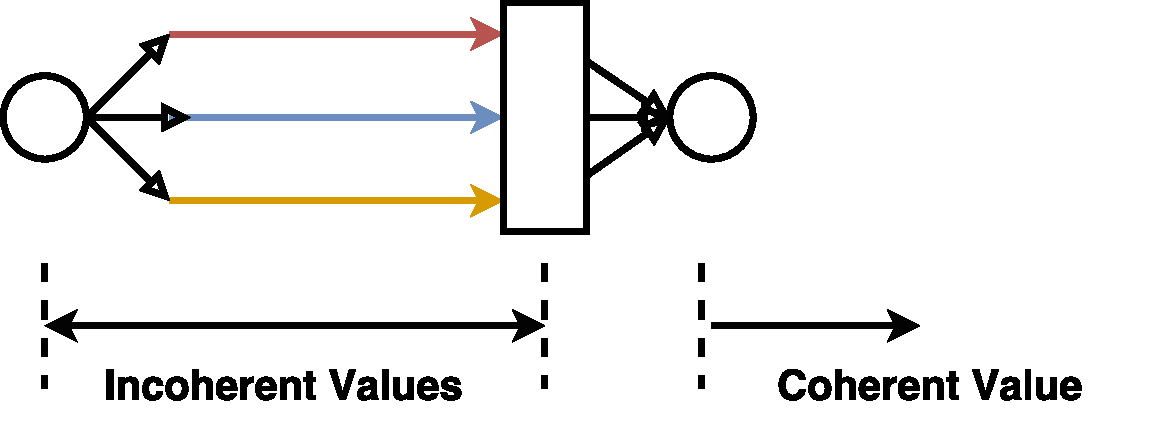
\includegraphics[width=0.50\textwidth]{incoherent.pdf}
    \caption{Values are split into each core's incoherent cache after APPROX and merged back to the coherent cache at MERGE}
    \label{fig:incoherent}
\end{figure}

We wanted to measure both the performance improvement and the potential
error of our incoherent cache approximation, unfortunately there isn't
an existing architecture or simulator which can evaluate such two fields at
once. Though we could model an existing simulator to do this, the work
would be too tedious as we are just doing a proof of concept, instead
what we did was modeled and yielded two separate versions of the input
program, one would be annotated with special functions calls that a
simulator can recognize and account for the corresponding cycle count,
and the other would be modified to take account for the effects of
actually using incoherent caches. Even though they are two separate 
programs, they share the same idea of doing the same approximation of
incoherent caching, just one is used to measure performance while the
other accounts for the potential output error.

In order to compute the performance benefit of our approximation
we used a PIN\cite{pin} based cache simulator. The simulator adds 
fixed cycle costs based on the level of cache from which the
data is accessed (three level cache modeled) and the coherence
state of the cacheline (MESI protocol modeled). The simulation
infrastructure is ready and has been in use for other research
for quite some time.

%TODO: Junhan, dont describe the simulation infrastructure here. Only describe the architecture over here
For our purpose we modeled a part of each core's L1 cache as incoherent
in the simulator, using PIN's routine instrumentation and identifying
special instructions that we marked in the code (particular blank or 
wrapper function calls which takes an argument that the simulator can 
then see marked as being stored in the incoherent cache), it can identify 
the data that needs to be stored in the incoherent cache and stores the
tag values in the cache. We also inserted blank \textit{do\_ merge()}
functions which tells the simulator the place to merge the incoherent
data in the cache and adds the corresponding cycle counts. In the 
coherent part of the program the coherent value is used while in the
incoherent part a separate incoherent value (marked as mentioned above)
is substituted and used, as we are not worrying about the error in
this program, we are only interested in the total cycle count after
it's execution, this approach is simple yet sufficient for us to use.
To be noted as we are using incoherence caches, it makes no sense
to keeping the synchronization guards aka locks guarding the shared
data, so we didn't account for any cycle counts for the locking and
unlocking of the critical sections guarding the shared data that
we put into the incoherent cache.

In order to evaluate the error in a program due to incoherent 
manipulation of data, for each shared data to be made incoherent,
we declared a separate array the size of the shared data multiplied
by the number of threads used in the program (which is either given
as a \#define or passed to the program as the first argument). Each 
thread spawned is given a unique tid going from 0,1... that is used
to access it's local private copy of the shared data. In place where
the APPROX instruction should be inserted the value of the data is
copied into the separate declared array and in place where the MERGE
instruction should be inserted an explicit merge is inserted to the
code which puts the merged data back to the original data. The 
incoherence part of the data is used with each thread's own local
copy of the data, while the coherent part remains the same using
the original value. While we are actually duplicating data in 
the program, the logical view of the duplication is basically
storing the shared data in an incoherent cache. The duplication of data
allows us to run the effect of no coherence on a native machine
that has coherence.

\section{Compiler Analysis} \label{sec:compiler}

In this project, we require compiler support to analysis the potential
shared variables that could be made incoherent. We used version 3.5.0
of the LLVM compiler framework\cite{llvm}, and restricted our analysis
to programs using the pthread library for parallel threading.
We implemented our passes as middle end passes for the LLVM IR language.

\subsection{Finding Potential Shared Variables}

The first thing to be done is to find potential shared variables that
can be approximated using incoherent cache. Shared variables should be
stored in the memory and not allocated as just a core's register, so 
the first approach is to find variables with the load-modify-store
pattern. We restricted our modify operations to be commutative so that
the merge later would be straightforward. Second, the shared variable
should be guarded within locks, and as we are restricting ourselves to
pthread programs, we only have to seek out the 
\texttt{phtread\_ mutex\_ lock()} and \texttt{pthread\_ mutex\_ unlock()} 
function calls and assume that the control flow guarded by pairs of
these two functions are in the critical section. So only access patterns
of load-modify-store inside the critical section are considered candidates
for approximation.

After finding the candidates we need to figure out the initial address of
the candidates, the value given to the load instruction might be generated
by a \texttt{getelementptr} instruction which calculate the offset address
in an array, by another \texttt{load} instruction which loads the address 
in the case of a pointer pointer, or a mixture of both, so in our pass we 
have to find the initial value used to calculate the address, so if the 
address is generated by another instruction we keep reverse tracking until 
we hit a globally declared variable which we recognizes as the origin of the
shared variable which we pass on to our further pass.

But before ending this pass we still have to do one more check, that is 
checking is the variable is used to determine the control flow of the
program, as if approximating a shared variable into a value that should
never be considered correct could result in non-deterministic control 
flow in the program and might result in a non-terminated program. Also
in our simulator the approximated data is never calculated so 
approximating the variable could lead to serious problems in our
simulator. We implemented this by finding all use cases of the candidate
and see if the value calculated using the candidate value is used in 
a branching statement or not, we can do a thorough analysis as to building
a tree of all values that are affected by this value and see if any of
them are used in a branching instruction, but this would be unreasonably
complicated because normally programs aren't this complicated as going down
just one or two levels down the tree is sufficient enough for most programs.

\subsection{Heuristics}

As mentioned before, we need to strategically place data
in the incoherent cache in order to contain the error in the 
program output to tolerable values. Thus we need compiler to do analysis 
to search for shared data in programs whose correctness is not critical to 
program quality. Given the list of potential candidates from the last
pass, we need to provide heuristics on identifying data that when
approximated estimated to not cause significant quality degradation.

\subsubsection{Estimating Importance of Program Variables}

Our first heuristics is to estimate the \emph{importance} of 
the shared variables. We say the importance are correlated to 
the number of uses of the shared variable in the program. This
can also build a tree of it's own including the uses of the values
calculated using the shared variable, but for the sake of simplicity
we only used the first level of uses of the shared data as a proxy 
to the importance of the shared variable.
\begin{figure}[h]
    \centering
    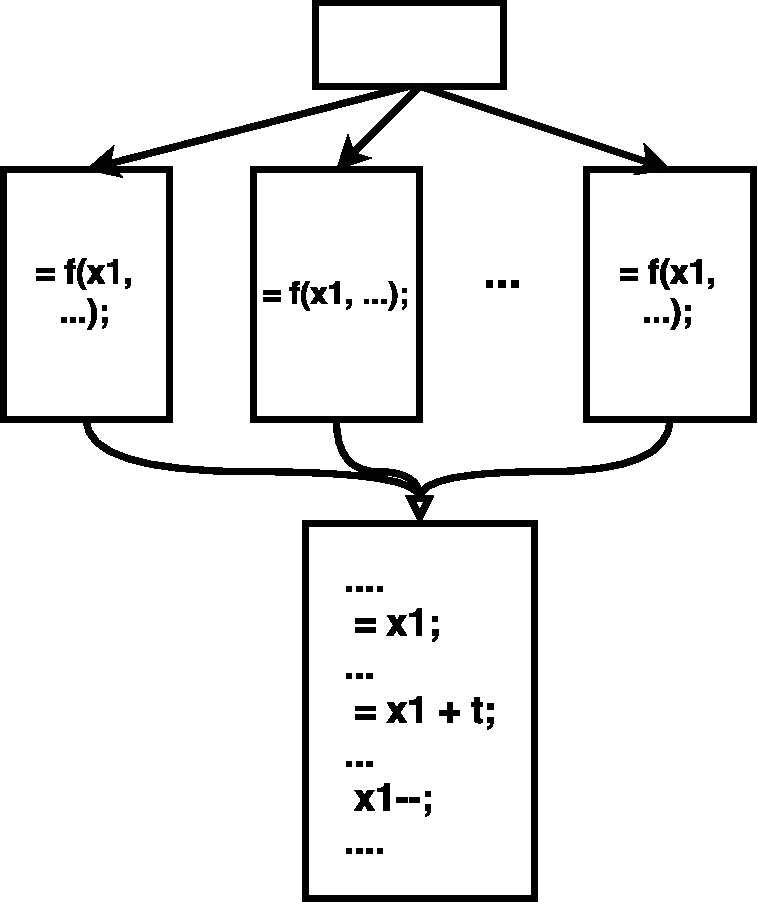
\includegraphics[width=0.40\textwidth]{Heuristic1.pdf}
    \caption{Heuristic1: Variables that are used less might be better approximation targets}
    \label{fig:h1}
\end{figure}

We think variables that are used less might be better approximation 
targets (lead to lesser quality degradation). For example the scan
operation which operates on an array will use the front data many
times then the data at the end, and also the data in the front
have a significant more impact on the overall quality of the 
scan operation while the last few data will only have influence
on the last few elements after the scan operation.

For each data passed in from the previous pass this pass counts all 
the uses of each respective data, given the aggressiveness of 
the approximation in this case the threshold of the number of 
uses for a variable, we can determine whether a variable should 
be approximated or not.

\subsubsection{Quality impact of approximating variables on infrequent branch paths}

We think that the quality impact of a certain shared variable can be estimated
by analyzing the place of use of the variable down the control flow. If the 
variable only appear on few paths, like only in one part of an unlikely taken
branch path, then it is not likely to cause significant quality degradation
on the program. More often then not the variable might not even be used by the
control flow of many instances of the program execution. Elsewise if a variable
is used on all paths down the control flow then it certainly would have a
quality impact on the given program.
\begin{figure}[h]
    \centering
    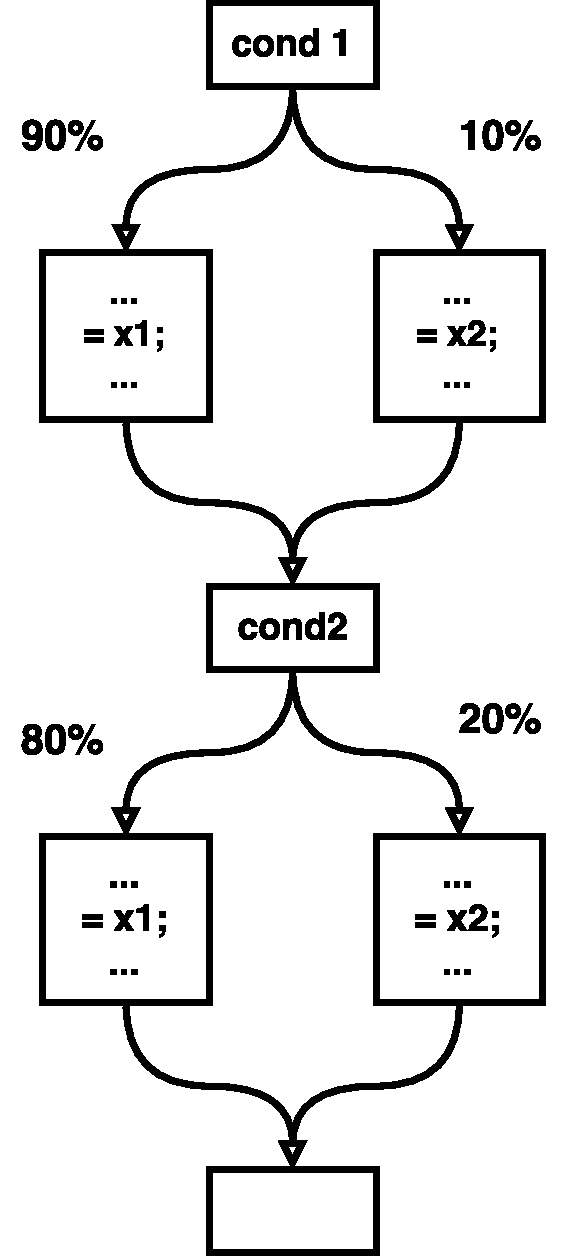
\includegraphics[width=0.30\textwidth]{Heuristic2.pdf}
    \caption{Heuristic2: Variables that appear only on few paths are not likely to cause significant quality degradation}
    \label{fig:h2}
\end{figure}

We implemented this pass by not only counting the uses of the potential shared
variables given, but also locate the use sites, that is in which basic block each
use of the value is in. We constructed a separated set data structure for each 
basic block and put all the used variable in the corresponding basic block's set.
We only counted the use of the load instruction and not the store instruction as 
sometimes the value itself is updated and sometimes it's used to figure out other
values, and each instance should be counted as one, so by ignoring store instruction
uses every instance of the use is only accounted for one time. After all the sets
are constructed, we traverse through the control flow graph and see which variable
is used only in certain path and which variable is used in all path. Given the
aggressiveness of approximation, in this case the path frequency where the variable
would be used, we can then determine which variable should be approximated or not.

\subsubsection{Detecting the Imbalance in Computation} \label{sec:h3}
As mentioned in section \ref{sec:mech}, our approximation mechanism involves placing
approximable data in an incoherent cache. In order to control the amount of 
error propogating through the program execution, our system provides the programmer 
with the option of \emph{merging} incoherent data. The merge operation operates upon
incoherent copies to produce the best approximation to the data had it been coherently
updated. 

For commutative operations (such as addition, multiplication, etc.) the merge operation 
can produce a completely precise result since the order of applying updates in a commutative 
update does not affect the result \cite{coup}. In order to add a dimension of approximation to
the merge operation, we implemented an approximate version of the merge operation. This idea is 
similar to the work done in \cite{paraprox} where reduction operation are made cheaper by 
reducing a subset of the total values and approximating the rest. 

Given such an approximate merge operation, we wanted our compiler pass to give us 
an idea of how much a particular variable could be approximated. In other words, we 
wanted a quantitative summary of the number of operands required by the approximate 
merge instruction for each approximation target in the program. We designed a heuristic 
to measure this quantity.

Our heuristic searches for imbalance in computations in different threads that could be
detected statically. For example in figure \ref{fig:h3}, the variable x is used more 
aggressively in the threads that are encapsulated by the rectangle than in other threads.
We can say that for this example variable x only requires the contribution of the first
two threads. Hence, our merge operation can factor in the results of the computation of
the first two threads alone. Only accounting for a subset of the values, allows the 
system to perform the merge operation faster at the expense of ignoring the results
of the other threads with few computations on the shared variable. 
\begin{figure}[h]
    \centering
    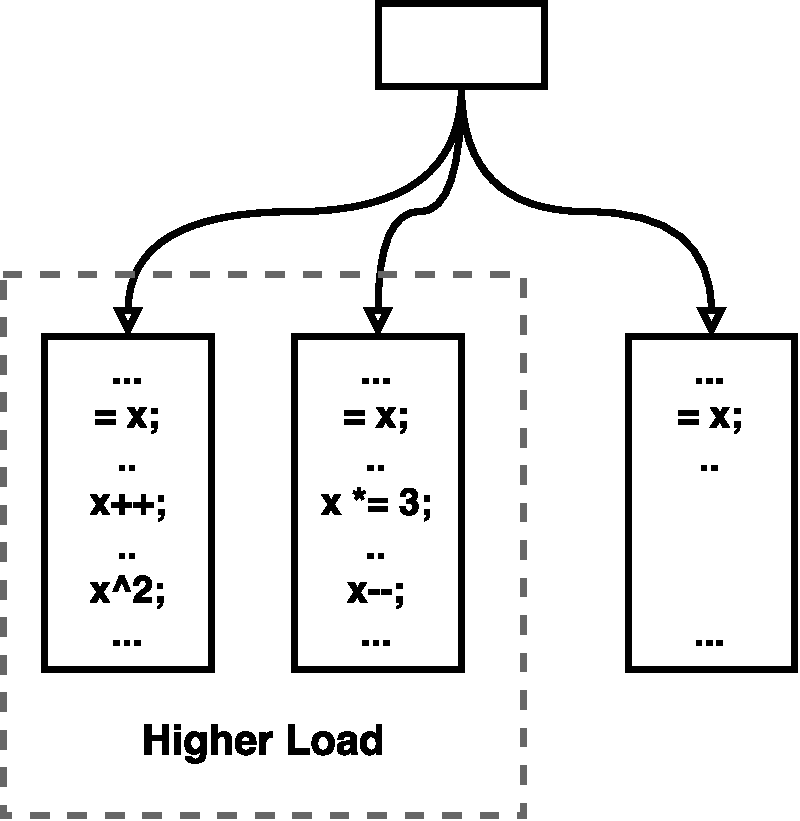
\includegraphics[width=0.40\textwidth]{Heuristic3.pdf}
    \caption{Heuristic3: Variables that are heavily operated upon only in a few threads do not need coherence for all threads}
    \label{fig:h3}
\end{figure}

This pass is implemented by first identifying all the calls to the 
\textit{pthread\_ create()} function and getting its third argument, which should
be the function that the pthread created the thread to launch on. Then for every
operations in the function counted how many uses of each of the shared 
variables, this serves as the indicator of the work amount of the current thread.



\section{Experimental Setup and Methodology} \label{sec:setup}

\begin{figure*}[h]
    \centering
    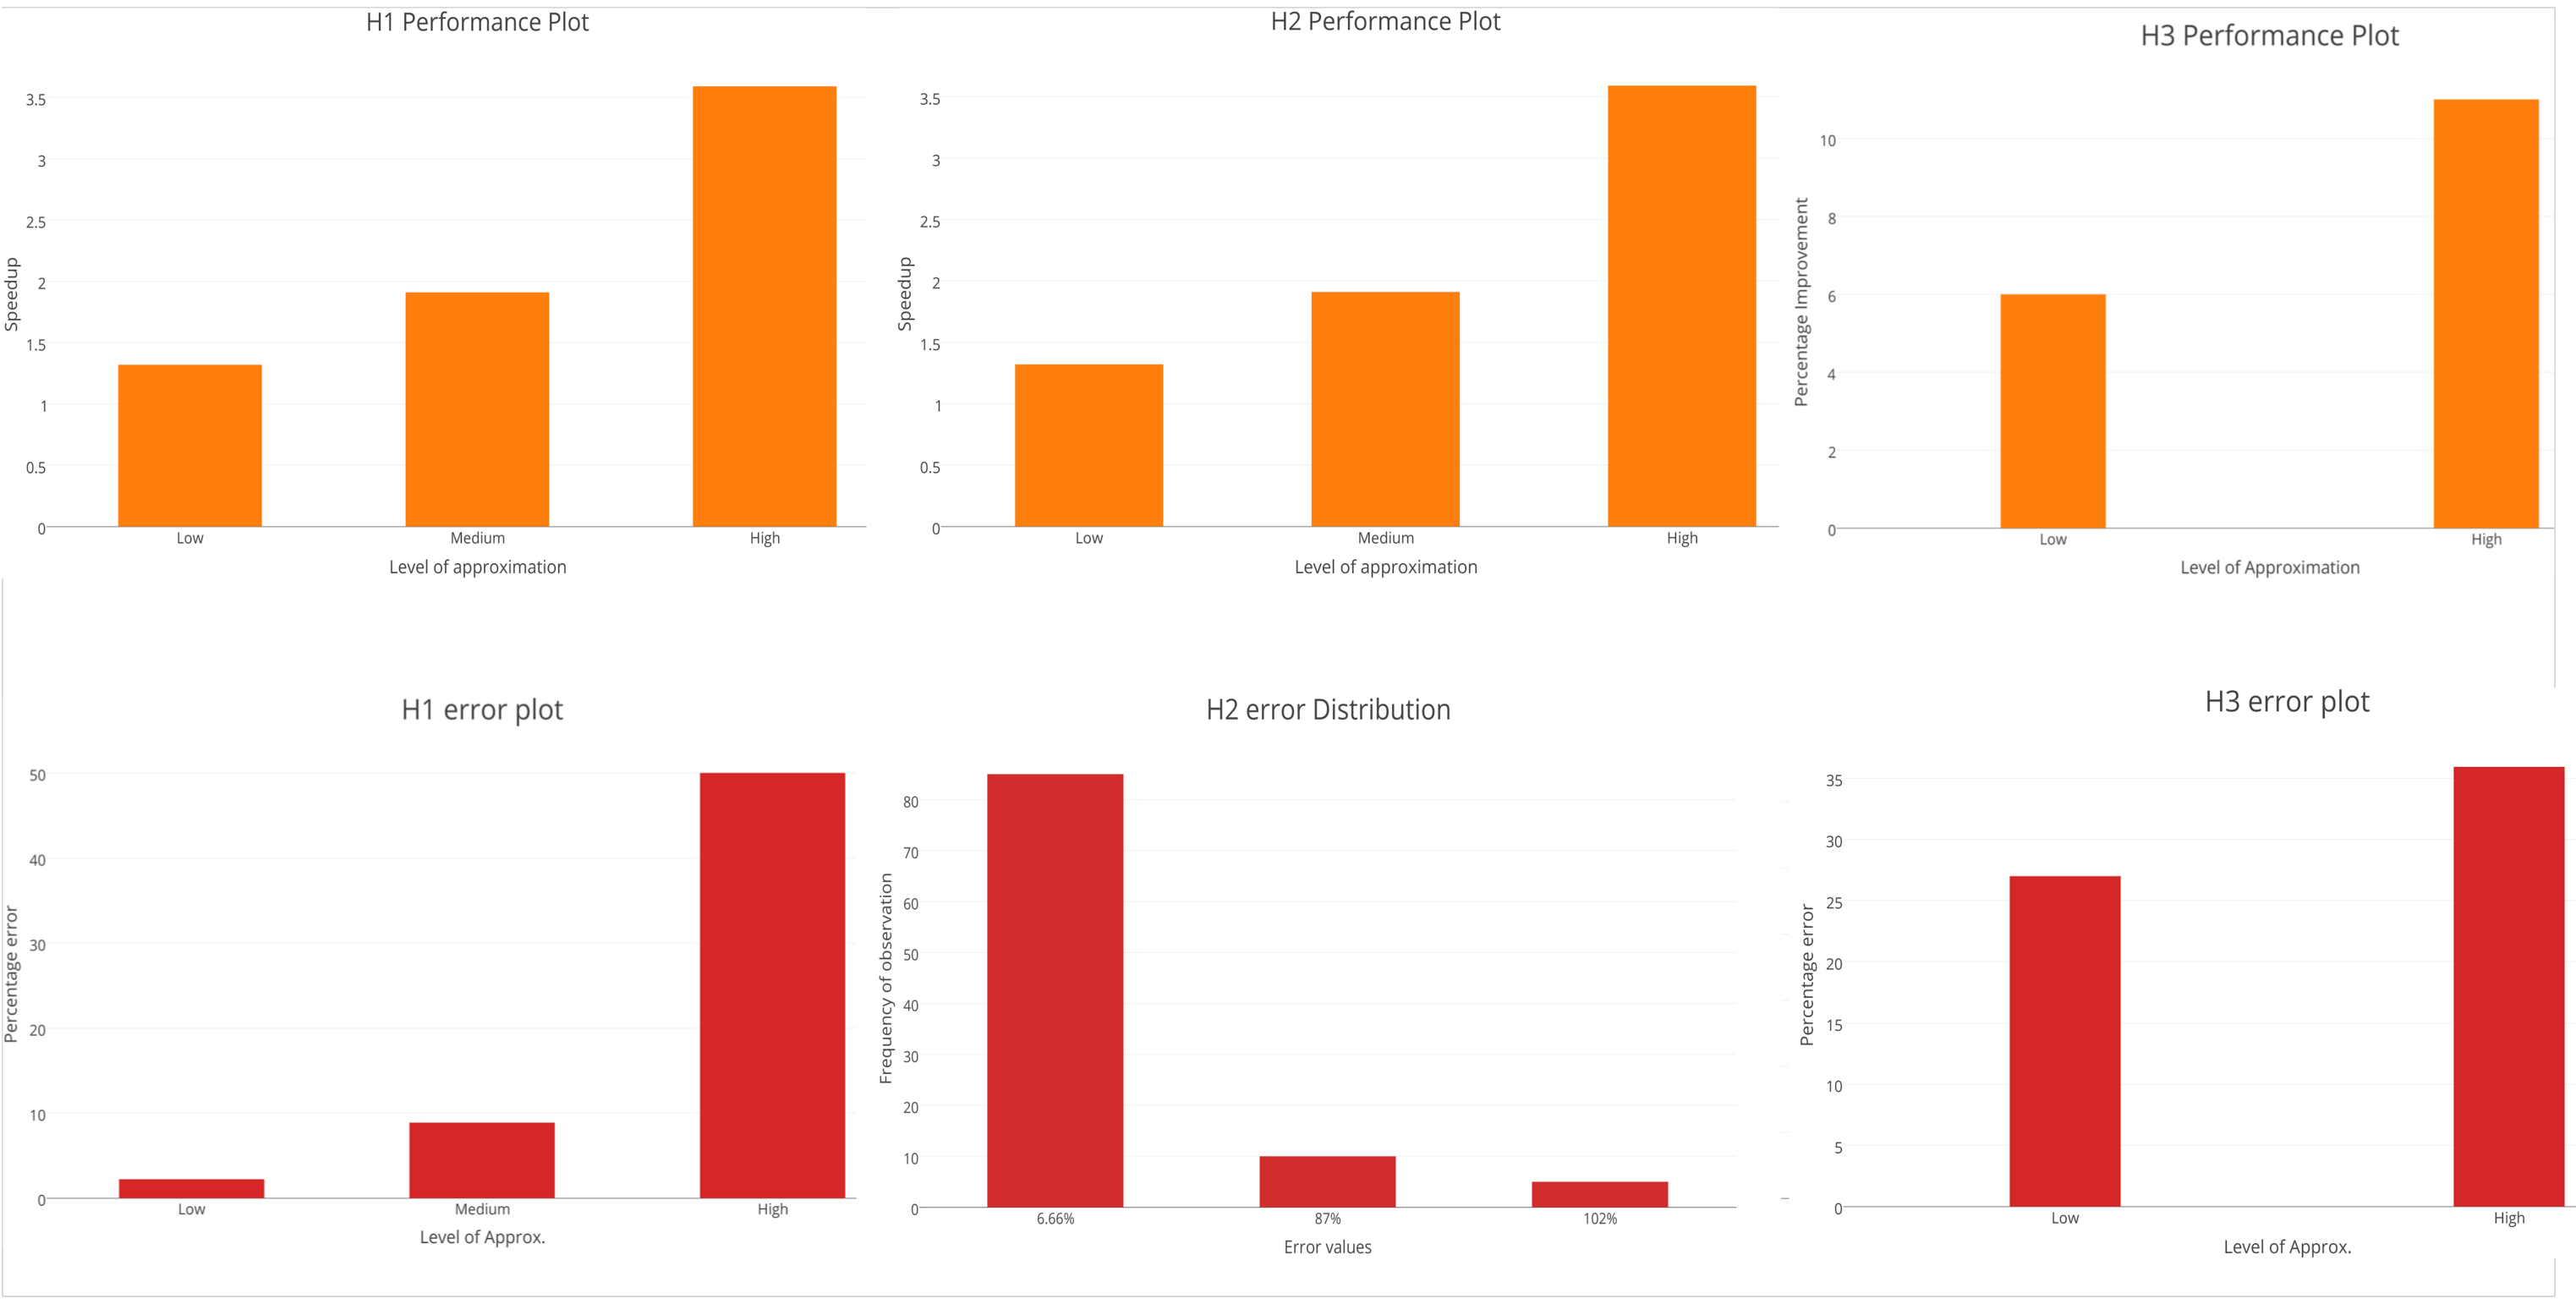
\includegraphics[width=0.95\textwidth]{result.png}
    \caption{Evaluation results on performance and error for the three proposed heuristics}
    \label{fig:result}
\end{figure*}

To evaluate the heuristics, we constructed several toy applications for our compiler 
passes to test out on. We modeled each of our toy application to correspond to a
particular heuristic that we proposed. That is for heuristic 1 we generated a toy
application where there are various random uses of the shared variables in the
sequential portion of the program following the parallel portion (which is a
common case for parallel programs, like in the map-reduce structure there is
a massive parallel \emph{map} stage followed by a sequential \emph{reduce} stage),
and for heuristic 2 we generated the sequential portion to include lots of different
control flows with a lot of if-else structures. For heuristic 3, as parallel
computations is not just single instruction multiple data (SIMD) type, we gave 
the \textit{pthread\_ create()} for each thread a different work function
with different work loads inside each of them.

%We evaluated our results by first running the original application directly for
%to get the precise output, then gave it to our PIN simulator to see the cycle
%counts for running this application.  After having the results for the precise
%version of the program, we gave it to our shared variables finding pass and
%passed it along to its corresponding heuristic pass. Upon using the information
%from the heuristic pass we tested various levels of approximation aggressiveness
%generating the various approximated version of the program into the performance
%and error evaluation version. We then gave the performance version to our simulator
%to get the cycle count of the approx

For the performance results, we used a PIN based simulator that
implemented a simple processor model. All non-memory instructions were assumed to
finish in one cycle. For memory instructions, our simulator modelled a detailed
three level cache heirarchy with the L1 and L2 being private to each core. We also 
modeled a directory based MESI cache coherence protocol. The cycle costs for 
accessing the memory heirarchy was based on average values reported for the 
Nehalem microarchitecture. In order to implement placing data in the incoherent cache, 
we had to slightly modify original code to insert special calls that our Pintool would
understand. The performance gain was then reported by computing the ratio of cycles (as
reported by the simulator) of the original version of the code over the modified (approximate) version. 

In order to calculate the error induced by incoherence, we used the concept of 
data duplication. Since there was no way to switch off coherence on our native machines, we
simulated the effect of incoherence by splitting the original shared variable as a thread
private copy. The operations on these private copies then are logically equivalent to cores
operating on incoherent data from their private caches. We implemented the merge operation discussed in 
section \ref{sec:h3} in the code by only combining the actual results of a 
few threads and approximating the rest. The error due to approximation was then 
reported as the percentage difference between the approximate (data-duplicated) version of the 
program and the precise version of the program. 

\section{Results} \label{sec:results}

We now discuss the performance and error results by approximating the
shared variable identified by our compiler pass based on the heuristics mentioned
in the previous section

Figure \ref{fig:result} shows the performance and error plots for applying each
heuristic independently. As can be seen in the figure, applying heuristic 1 and 2
gives considerable improvement in the parallel portion of the program by speeding 
up the computations by upto 3.5 times the precise version of the program. We observe
the same performance improvement for these two heuristics because the parallel 
part of the test program was the same for both experiments. The performance benefit
in this case can be attributed to the reduced data movement between cores in the approximate
version of the program. A reduction in the coherence traffic is also a contributor in the 
performance speedup. The performance results also indicate that increasing the approximation 
by placing more data in the incoherent cache results in greater speedup which is an 
intuitive result. 

The difference in the test programs for heuristics 1 and 2 was in the post parallel phase 
of the computation. For heuristic 1, the post parallel phase only involved simple uses 
of the shared variable as described in figure \ref{fig:h1}. The error plots for heuristic 1
illustrates the increasing disadvantage of keeping more data in the incoherent cache with
error rates of upto 50\%. These plots show the performance-accuracy tradeoff space that is
opened up by approximate computing.

For the error induced by approximating the suggestions of heuristic 2 we present a different 
view of error data. The test program for heuristic 2 had computations in which some variables 
were only used in branches of the code which were executed very infrequently. An example computation
can be seen in figure \ref{fig:h2}. We report the distribution of error for approximating 
a variable that only appeared in infrequently executed branches as observed in 100 runs of the
experiment. As can be seen in the 
error plot for heuristic 2, we observe a very small error ($<$6\%) most of the time (85\%).
Larger values of errors are only observed with a small frequency and, hence, the expected
value of error due to approximation is expected to be low.

The test program for testing the efficacy of heuristic 3 was similar to the example depicted
in figure \ref{fig:h3}. The approximation in this program involved operating upon the
result of a subset of the total threads and approximating the results of other threads. We 
tested the program for cases when a third of the threads were merged (titled low approximation)
and when two thirds of the thread values were merged (titled high approximation). The cycle
cost for the merge operation was also adjusted to account for faster merge operations in
the high approximation case. The performance benefit of these two approximations is not 
significantly high relative to the other cases we have seen so far (only 
12\% performance improvement of high approximation over precise version). An explanation 
of this behavior could be that the merge operation is not a significant bottleneck in 
the parallel program and, hence, optimizing it yielded minimal performance improvement. 
This result shows that the performance improvement is maximum when data movement is 
limited as evidenced by the results for heuristics 1 and 2. The error plot for heuristic 3 
shows significant error degradation even for low level of approximation. This result
was expected since we are completely ignoring the contribution of a few threads in the 
computation of the approximate value. In summary, our results show that tuning the 
number of operands in the approximate merge operation can be dangerous since it causes
significant errors in the program for marginal performance improvement

The main theme that we wished to portray in all our results was that the 
performance and quality degradation of that we observed in our programs were in
the same direction as predicted by our three heuristics. Even though our heuristics cannot
select approximation targets by reasoning the quality degradation quantitatively, our 
results show that a qualitative estimation of error can be effective in applying 
approximations to programs with sufficient tolerance to errors in program values. 

 
\section{Limitations of our work} \label{sec:limitations}

There are a few limitations in our method for detecting approximation targets and these
limitations are useful in understanding the position of our contribution in 
relation to other work done in approximate computing. The two primary limitations 
of our work are:
\begin{itemize}
\item The inability to provide quality guarantees
\item The inability to reason about dynamic aspects of programs
\end{itemize}

\subsection{Quality guarantees}

In this work, we only focus on finding the approximation targets by
qualitative reasoning. We use heuristics to detect approximation targets that 
would, hopefully, not cause too much quality degradation. However, this heuristic
is not guaranteed to work in all cases. One could imagine examples wherein certain
data are absolutely critical to program correctness. Additionally, it is quite possible
that these data values are only accessed a few times in the program's lifetime (this
is a good approximation target as per our heurstic). For example, a pointer value 
should not be approximated even if it altered just once in the program since that
might result in a segmentation fault. 

The root cause of this problem is our inability to tease out information of 
importance of data values from data flow analysis. The assumption that
the usage of a value will be correlated with its importance in the result
is not always true and, hence, no compiler analysis can get such information. 
Therefore, it is imperative that the programmer conveys information about 
precision requirements of certain values to the compiler\cite{approx}\cite{enerJ}\cite{rely}.
Our compiler pass armed with programmer annotations of precise data can provide a 
more solid guarantee on program quality by never approximating the precise values.

\subsection{Dynamic information}

Our compiler passes work for programs with very specific characteristics (the patterns
we search for in each of our heuristics). Our analysis ignores the effects of 
dynamic code information such as loops and branch hit rates. The importance of 
a value finally depends upon the number of times it is used and manipulated 
during an actual run of the program. Since our pass does not have access to 
dynamic information (such as from profiling) we cannot find approximation targets that
are hidden inside loops. With the help of information from profiling the program 
we can devise more sophesticated heuristics based upon dynamic information to 
find more approximation targets.
 

\section{Conclusion}\label{sec:conclusion}

In this work, we took one step further in the direction of applying approximate computing
to improve the performance of parallel programs. We showed the promise of 
approximating data values by introducing an incoherent cache. The main contribution
of this work was to show that a compiler pass could be used to detect the 
best approximation targets that would yield good performance improvements at minimal
program quality degradation. To this end, we designed and tested a couple of 
heuristics to find the pareto optimal points in the performance-accuracy tradeoff space.
In conclusion, we believe our work is a useful tool in finding approximation targets
in the absence of code annotations to mark approximable data and dynamic profile information. 



% And in order to find potential
%good values to approximate, we built compiler passes that first identified the 
%shared variables and then applied heuristics to estimate the potential impact of 
%the variable with uses count, path appearance estimate and imbalance between threads.
%Our results showed a decent improvement for our toy applications while sustaining 
%minimal error rate if not approximated too aggressively.
%
%Limitations on our approach is as we are only doing a static analysis of the program,
%we have no way of knowing any run-time dynamic information. Other systems such as 
%\cite{green}\cite{chisel} have done code profiling to get an idea on the dynamic 
%aspects of the code, \cite{ibm}\cite{helixup}\cite{paraprox}\cite{green} all used 
%run time frameworks to dynamically adjust the approximating rate based on the 
%resulting error rate, rewinding and redoing the precise version of the program 
%if the approximate version's result is not ideal ensuring there is a upper
%bound on the quality degradation of the approximated program. Future work can be 
%done here to also build our own run time framework or integrate with one of the 
%available frameworks to provide the dynamic analysis capabilities and rewind on 
%unacceptable error ratio options that we lack now.
%
%Future work can also be done by letting the programmer write special code annotations
%to tell our compiler which variable is a good candidate for approximation as in
%\cite{enerJ}\cite{accept}\cite{chisel}. The programmer doesn't need to indicate 
%each and every variable to be approximated, by just telling a potential candidate 
%future work can be done using inductions in the ways of \cite{chisel}\cite{stochastic}
%tracking the uses and users of the given variable to find a good approximate 
%candidate.

\section{Contributions}

Junhan Zhou: 50\%\\
Vignesh Balaji: 50\%




% An example of a floating figure using the graphicx package.
% Note that \label must occur AFTER (or within) \caption.
% For figures, \caption should occur after the \includegraphics.
% Note that IEEEtran v1.7 and later has special internal code that
% is designed to preserve the operation of \label within \caption
% even when the captionsoff option is in effect. However, because
% of issues like this, it may be the safest practice to put all your
% \label just after \caption rather than within \caption{}.
%
% Reminder: the "draftcls" or "draftclsnofoot", not "draft", class
% option should be used if it is desired that the figures are to be
% displayed while in draft mode.
%
%\begin{figure}[!t]
%\centering
%\includegraphics[width=2.5in]{myfigure}
% where an .eps filename suffix will be assumed under latex, 
% and a .pdf suffix will be assumed for pdflatex; or what has been declared
% via \DeclareGraphicsExtensions.
%\caption{Simulation results for the network.}
%\label{fig_sim}
%\end{figure}

% Note that the IEEE typically puts floats only at the top, even when this
% results in a large percentage of a column being occupied by floats.


% An example of a double column floating figure using two subfigures.
% (The subfig.sty package must be loaded for this to work.)
% The subfigure \label commands are set within each subfloat command,
% and the \label for the overall figure must come after \caption.
% \hfil is used as a separator to get equal spacing.
% Watch out that the combined width of all the subfigures on a 
% line do not exceed the text width or a line break will occur.
%
%\begin{figure*}[!t]
%\centering
%\subfloat[Case I]{\includegraphics[width=2.5in]{box}%
%\label{fig_first_case}}
%\hfil
%\subfloat[Case II]{\includegraphics[width=2.5in]{box}%
%\label{fig_second_case}}
%\caption{Simulation results for the network.}
%\label{fig_sim}
%\end{figure*}
%
% Note that often IEEE papers with subfigures do not employ subfigure
% captions (using the optional argument to \subfloat[]), but instead will
% reference/describe all of them (a), (b), etc., within the main caption.
% Be aware that for subfig.sty to generate the (a), (b), etc., subfigure
% labels, the optional argument to \subfloat must be present. If a
% subcaption is not desired, just leave its contents blank,
% e.g., \subfloat[].


% An example of a floating table. Note that, for IEEE style tables, the
% \caption command should come BEFORE the table and, given that table
% captions serve much like titles, are usually capitalized except for words
% such as a, an, and, as, at, but, by, for, in, nor, of, on, or, the, to
% and up, which are usually not capitalized unless they are the first or
% last word of the caption. Table text will default to \footnotesize as
% the IEEE normally uses this smaller font for tables.
% The \label must come after \caption as always.
%
%\begin{table}[!t]
%% increase table row spacing, adjust to taste
%\renewcommand{\arraystretch}{1.3}
% if using array.sty, it might be a good idea to tweak the value of
% \extrarowheight as needed to properly center the text within the cells
%\caption{An Example of a Table}
%\label{table_example}
%\centering
%% Some packages, such as MDW tools, offer better commands for making tables
%% than the plain LaTeX2e tabular which is used here.
%\begin{tabular}{|c||c|}
%\hline
%One & Two\\
%\hline
%Three & Four\\
%\hline
%\end{tabular}
%\end{table}


% Note that the IEEE does not put floats in the very first column
% - or typically anywhere on the first page for that matter. Also,
% in-text middle ("here") positioning is typically not used, but it
% is allowed and encouraged for Computer Society conferences (but
% not Computer Society journals). Most IEEE journals/conferences use
% top floats exclusively. 
% Note that, LaTeX2e, unlike IEEE journals/conferences, places
% footnotes above bottom floats. This can be corrected via the
% \fnbelowfloat command of the stfloats package.







% trigger a \newpage just before the given reference
% number - used to balance the columns on the last page
% adjust value as needed - may need to be readjusted if
% the document is modified later
%\IEEEtriggeratref{8}
% The "triggered" command can be changed if desired:
%\IEEEtriggercmd{\enlargethispage{-5in}}

% references section

% can use a bibliography generated by BibTeX as a .bbl file
% BibTeX documentation can be easily obtained at:
% http://mirror.ctan.org/biblio/bibtex/contrib/doc/
% The IEEEtran BibTeX style support page is at:
% http://www.michaelshell.org/tex/ieeetran/bibtex/
%\bibliographystyle{IEEEtran}
% argument is your BibTeX string definitions and bibliography database(s)
%\bibliography{IEEEabrv,../bib/paper}
%
% <OR> manually copy in the resultant .bbl file
% set second argument of \begin to the number of references
% (used to reserve space for the reference number labels box)
\begin{thebibliography}{11}

\bibitem{tile}
Bob Doud, Accelerating the Data Plane With the TILE-Mx Manycore Processor, 
http://www.tilera.com/files/drim\_\_ EZchip\_LinleyDataCenterConference\_Feb2015\_7671.pdf

\bibitem{ibm}
L Renganarayana, V Srinivasan, R Nair, D Prener, C Blundell,Relaxing synchronization for performance and insight,Technical Report RC25256, IBM 

\bibitem{helixup}
Simone Campanoni, Glenn Holloway, Gu-Yeon Wei, and David Brooks. “HELIX-UP: Relaxing
Program Semantics to Unleash Parallelization,” in Proceedings of the 2015 International
Symposium on Code Generation and Optimization (CGO ’15), February 2015.

\bibitem{coup}
Guowei Zhang, Webb Horn, and Daniel Sanchez. 2015. Exploiting commutativity to reduce the cost of updates to shared data in cache-coherent systems. In Proceedings of the 48th International Symposium on Microarchitecture (MICRO-48). ACM, New York, NY, USA, 13-25. 

\bibitem{pin}
Chi-Keung Luk, Robert Cohn, Robert Muth, Harish Patil, Artur Klauser, Geoff Lowney, Steven Wallace, Vijay Janapa Reddi, and Kim Hazelwood. 2005. Pin: building customized program analysis tools with dynamic instrumentation. SIGPLAN Not. 40, 6 (June 2005), 190-200.

\bibitem{paraprox}
Mehrzad Samadi, Davoud Anoushe Jamshidi, Janghaeng Lee, and Scott Mahlke. 2014. Paraprox: pattern-based approximation for data parallel applications. In Proceedings of the 19th international conference on Architectural support for programming languages and operating systems (ASPLOS '14). ACM, New York, NY, USA, 35-50. 

\bibitem{llvm}
Chris Lattner and Vikram Adve. 2004. LLVM: A Compilation Framework for Lifelong Program Analysis \& Transformation. In Proceedings of the international symposium on Code generation and optimization: feedback-directed and runtime optimization (CGO '04). IEEE Computer Society, Washington, DC, USA, 75-.

\bibitem{green}
Woongki Baek and Trishul M. Chilimbi. 2010. Green: a framework for supporting energy-conscious programming using controlled approximation. SIGPLAN Not. 45, 6 (June 2010), 198-209. 

\bibitem{enerJ}
Adrian Sampson, Werner Dietl, Emily Fortuna, Danushen Gnanapragasam, Luis Ceze, and Dan Grossman. 2011. EnerJ: approximate data types for safe and general low-power computation. In Proceedings of the 32nd ACM SIGPLAN Conference on Programming Language Design and Implementation (PLDI '11)

\bibitem{accept}
Sampson, Adrian, et al. "Accept: A programmer-guided compiler framework for practical approximate computing." University of Washington Technical Report UW-CSE-15-01 1 (2015)

\bibitem{chisel}
Sasa Misailovic, Michael Carbin, Sara Achour, Zichao Qi, and Martin C. Rinard. 2014. Chisel: reliability- and accuracy-aware optimization of approximate computational kernels. In Proceedings of the 2014 ACM International Conference on Object Oriented Programming Systems Languages \& Applications (OOPSLA '14) 

\bibitem{approx}
Eric Schkufza, Rahul Sharma, and Alex Aiken. “Stochastic optimization of floating-point
programs with tunable precision,” in Proceedings of the 35th ACM SIGPLAN Conference on
Programming Language Design and Implementation (PLDI ’14), June 2014.

\bibitem{rely}
Lakshminarayanan Renganarayana, Vijayalakshmi Srinivasan, Ravi Nair, and Daniel Prener. 2012. Programming with relaxed synchronization. In Proceedings of the 2012 ACM workshop on Relaxing synchronization for multicore and manycore scalability (RACES '12)

\end{thebibliography}
% that's all folks
\end{document}


